\documentclass{beamer}



\usepackage{pgfplots}
\pgfplotsset{compat=1.17}

\usepackage{animate}
\usepackage[spanish]{babel}
\usepackage[utf8]{inputenc}
\usepackage{amsmath}
\usepackage{pgfplots}
 \usepackage{graphicx}
\usetheme{Madrid}
\title{Interpolación Lineal y de lagrange}

\author{H.D Salinas \\
Curso de métodos computacionales\\
Universidad de Antioquia\\}


\date{\today}

\begin{document}

\begin{frame}
  \titlepage
\end{frame}


\begin{frame}{Linear interpolation formula}
    
        The linear interpolation formula can be derived from the equation of a straight line that passes through two given points $(x_i,y_i)$ and $(x_{i+1},y_{i+1})$:
    
    $(x_{i+1},y_{i+1})$
        \begin{align*}
            y &= mx + b \\
            m &= \frac{y_{i+1}-y_i}{x_{i+1}-x_i} \\            
            b &= y_i-\frac{y_{i+1}-y_i}{x_{i+1}-x_i}x_i \\
            y &= \frac{y_{i+1}-y_i}{x_{i+1}-x_i}x+b \\
        \end{align*}

        This formula can be applied for any value of $x$ between the endpoints of the interval.
\end{frame}

\begin{frame}{Linear interpolation formula}
    \begin{block}{Notation}
        We can write the linear interpolation formula as:
        \begin{align}
        %$$  
        f(x)\approx y = &\frac{y_{i+1}-y_i}{x_{i+1}-x_i}(x-x_i) + y_i \\
        =&\frac{y_{i+1}-y_i}{x_{i+1}-x_i}x+\left[y_i-\frac{y_{i+1}-y_i}{x_{i+1}-x_i}x_i\right] \\
        %$$
        \end{align}
        where $(x_1,y_1)$ and $(x_2,y_2)$ are the two given points and $f(x)$ is the estimated value of the function at $x$.
    \end{block}
\end{frame}


\begin{frame}


\end{frame}


\begin{frame}{Interpolación}

\begin{block}{Teorema}
Suponga que f esta definida en a, b, para cada $\epsilon<0$, entonces
existe un polinomio $P(x)$ que cumple:
    \begin{equation}
    |f(x)-P(x)|<\epsilon
    \end{equation}
    \end{block}
    
    \begin{center}
    \begin{figure}
    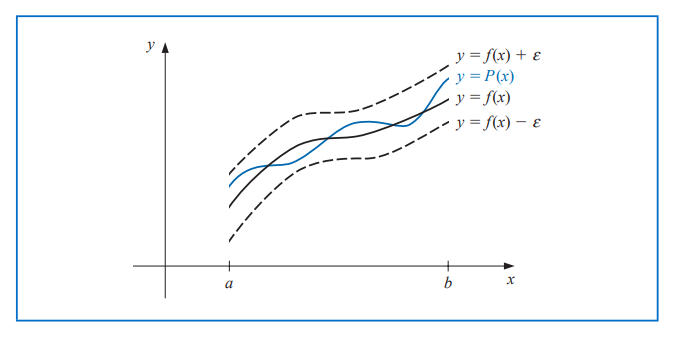
\includegraphics[width=0.7\textwidth]{lagrange01.png}
    \caption{Interpolacion lagrange.} 
    \end{figure} 
    \end{center}
\end{frame}


\begin{frame}{Interpolacion Lagrange}
¿cómo podemos garantizar un polinomio que pase por los dos puntos?
   \begin{center}
     \scalebox{0.8}{
    \begin{tikzpicture}
      \begin{axis}[
        xlabel=$x$,
        ylabel=$y$,
        xmin=0,
        xmax=3,
        ymin=0,
        ymax=10
      ]     
   %   \addplot[mark=*] coordinates {(-1.7693,0)};
    %  \addplot[mark=*] coordinates {(0,2)};     
    %  \addplot[red,samples=100] {-2*x+2};
      \addplot[mark=*] coordinates {(1,1)};
      \addplot[mark=*] coordinates {(2.,6)};      
      \addplot[dashed] coordinates {(0,-5) (0,5)};
      \addplot[dashed] coordinates {(-5,0) (5,0)};     
     
      \end{axis}
    \end{tikzpicture}}
  \end{center}
    
\end{frame}

\begin{frame}{Interpolación Lagrange}
¿cómo podemos garantizar un polinomio que pase por los dos puntos?
   \begin{center}
     \scalebox{0.8}{
    \begin{tikzpicture}
      \begin{axis}[
        xlabel=$x$,
        ylabel=$y$,
        xmin=0,
        xmax=3,
        ymin=0,
        ymax=10
      ]     
   %   \addplot[mark=*] coordinates {(-1.7693,0)};
    %  \addplot[mark=*] coordinates {(0,2)};     
    %  \addplot[red,samples=100] {-2*x+2};
     \addplot[blue,samples=100] {x^3-2*x+2};
    \addplot[mark=*] coordinates {(1,1)};
      \addplot[mark=*] coordinates {(2.,6)};      
      \addplot[dashed] coordinates {(0,-5) (0,5)};
      \addplot[dashed] coordinates {(-5,0) (5,0)};     
     
      \end{axis}
    \end{tikzpicture}}
  \end{center}
    \pause
    \[
    P(x) = y_0 \mathscr{L}_0(x) + y_1 \mathscr{L}_1(x)
    \]
\end{frame}

\begin{frame}{Interpolación de Lagrange para dos puntos}
    Si queremos interpolar una función en dos puntos $(x_0,y_0)$ y $(x_1,y_1)$, el polinomio de interpolación de Lagrange es de grado 1 y se obtiene así:
    \[
    P(x) = f(x_0) \mathscr{L}_0(x) + f(x_1) \mathscr{L}_1(x)
    \]
    donde
    \[
    \mathscr{L}_0(x) = \frac{x-x_1}{x_0-x_1} \quad \text{y} \quad \mathscr{L}_1(x) = \frac{x-x_0}{x_1-x_0}
    \]
    Expandiendo los productos se tiene que:
    \[
    P(x) = y_0 \left(\frac{x-x_1}{x_0-x_1} \right)+ y_ 1 \left(\frac{x-x_0}{ x _  1 - x _  0} \right)
    \]
    Note que : $\mathscr{L}_0(x_0)=1$, $\mathscr{L}_0(x_1)=0$, $\mathscr{L}_1(x_0)=0$, $\mathscr{L}_1(x_1)=1$
    
\end{frame}


\begin{frame}{Interpolación de Lagrange}
Dado un conjunto de $n+1$ puntos donde todos los $x_j$ se asumen distintos, el polinomio interpolador en la forma de Lagrange es la combinación lineal de bases polinómicas de Lagrange:
    \[
    P(x) = \sum_{k=0}^n f(x_k) \mathscr{L}_{n,k}(x)
    \]
    donde
    \[
    \mathscr{L}_{n,k}(x) = \prod_{k=0,i\neq k}^k \frac{x-x_i}{x_k-x_i}
    \]
    
\end{frame}

\begin{frame}{Grafica del polinomio de lagrange}
 \begin{center}
    \begin{figure}
    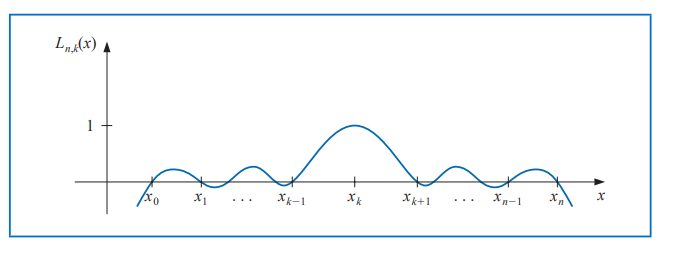
\includegraphics[width=1.0\textwidth]{lagrange02.png}
    \caption{Interpolacion lagrange.} 
    \end{figure} 
    \end{center}
\end{frame}

\begin{frame}{Error en el polinomio de lagrange}
 \[
    P(x) = \sum_{k=0}^n f(x_k) \mathscr{L}_{n,k}(x)
    \]
    donde
    \[
    \mathscr{L}_{n,k}(x) = \prod_{k=0,i\neq k}^k \frac{x-x_i}{x_k-x_i}
    \]

\[
f(x) = P(x) + \frac{f^{n+1}(\xi(x))}{(n+1)!} (x-x_0)(x-x_1)...(x-x_n)
\]

donde P(x) es el polinomio de interpolación
\end{frame}


\begin{frame}{Referencias}
\begin{itemize}
 \item Burden, R. L., Faires, J. D., & Burden, A. M. (2016). Análisis numérico (10a ed.). Cengage Learning.3

\end{itemize}
\end{frame}


\end{document}